% Options for packages loaded elsewhere
\PassOptionsToPackage{unicode}{hyperref}
\PassOptionsToPackage{hyphens}{url}
%
\documentclass[
  english,
  ,pub,floatsintext]{apa6}
\usepackage{amsmath,amssymb}
\usepackage{lmodern}
\usepackage{ifxetex,ifluatex}
\ifnum 0\ifxetex 1\fi\ifluatex 1\fi=0 % if pdftex
  \usepackage[T1]{fontenc}
  \usepackage[utf8]{inputenc}
  \usepackage{textcomp} % provide euro and other symbols
\else % if luatex or xetex
  \usepackage{unicode-math}
  \defaultfontfeatures{Scale=MatchLowercase}
  \defaultfontfeatures[\rmfamily]{Ligatures=TeX,Scale=1}
\fi
% Use upquote if available, for straight quotes in verbatim environments
\IfFileExists{upquote.sty}{\usepackage{upquote}}{}
\IfFileExists{microtype.sty}{% use microtype if available
  \usepackage[]{microtype}
  \UseMicrotypeSet[protrusion]{basicmath} % disable protrusion for tt fonts
}{}
\makeatletter
\@ifundefined{KOMAClassName}{% if non-KOMA class
  \IfFileExists{parskip.sty}{%
    \usepackage{parskip}
  }{% else
    \setlength{\parindent}{0pt}
    \setlength{\parskip}{6pt plus 2pt minus 1pt}}
}{% if KOMA class
  \KOMAoptions{parskip=half}}
\makeatother
\usepackage{xcolor}
\IfFileExists{xurl.sty}{\usepackage{xurl}}{} % add URL line breaks if available
\IfFileExists{bookmark.sty}{\usepackage{bookmark}}{\usepackage{hyperref}}
\hypersetup{
  pdftitle={Dog and owner characteristics predict training success},
  pdfauthor={Jeffrey R. Stevens1, London M. Wolff1, Megan Bosworth1, \& Jill Morstad2},
  pdflang={en-EN},
  pdfkeywords={Canine Good Citizen test, dog, obedience, training},
  hidelinks,
  pdfcreator={LaTeX via pandoc}}
\urlstyle{same} % disable monospaced font for URLs
\usepackage{graphicx}
\makeatletter
\def\maxwidth{\ifdim\Gin@nat@width>\linewidth\linewidth\else\Gin@nat@width\fi}
\def\maxheight{\ifdim\Gin@nat@height>\textheight\textheight\else\Gin@nat@height\fi}
\makeatother
% Scale images if necessary, so that they will not overflow the page
% margins by default, and it is still possible to overwrite the defaults
% using explicit options in \includegraphics[width, height, ...]{}
\setkeys{Gin}{width=\maxwidth,height=\maxheight,keepaspectratio}
% Set default figure placement to htbp
\makeatletter
\def\fps@figure{htbp}
\makeatother
\setlength{\emergencystretch}{3em} % prevent overfull lines
\providecommand{\tightlist}{%
  \setlength{\itemsep}{0pt}\setlength{\parskip}{0pt}}
\setcounter{secnumdepth}{-\maxdimen} % remove section numbering
% Make \paragraph and \subparagraph free-standing
\ifx\paragraph\undefined\else
  \let\oldparagraph\paragraph
  \renewcommand{\paragraph}[1]{\oldparagraph{#1}\mbox{}}
\fi
\ifx\subparagraph\undefined\else
  \let\oldsubparagraph\subparagraph
  \renewcommand{\subparagraph}[1]{\oldsubparagraph{#1}\mbox{}}
\fi
% Manuscript styling
\usepackage{upgreek}
\captionsetup{font=singlespacing,justification=justified}

% Table formatting
\usepackage{longtable}
\usepackage{lscape}
% \usepackage[counterclockwise]{rotating}   % Landscape page setup for large tables
\usepackage{multirow}		% Table styling
\usepackage{tabularx}		% Control Column width
\usepackage[flushleft]{threeparttable}	% Allows for three part tables with a specified notes section
\usepackage{threeparttablex}            % Lets threeparttable work with longtable

% Create new environments so endfloat can handle them
% \newenvironment{ltable}
%   {\begin{landscape}\begin{center}\begin{threeparttable}}
%   {\end{threeparttable}\end{center}\end{landscape}}
\newenvironment{lltable}{\begin{landscape}\begin{center}\begin{ThreePartTable}}{\end{ThreePartTable}\end{center}\end{landscape}}

% Enables adjusting longtable caption width to table width
% Solution found at http://golatex.de/longtable-mit-caption-so-breit-wie-die-tabelle-t15767.html
\makeatletter
\newcommand\LastLTentrywidth{1em}
\newlength\longtablewidth
\setlength{\longtablewidth}{1in}
\newcommand{\getlongtablewidth}{\begingroup \ifcsname LT@\roman{LT@tables}\endcsname \global\longtablewidth=0pt \renewcommand{\LT@entry}[2]{\global\advance\longtablewidth by ##2\relax\gdef\LastLTentrywidth{##2}}\@nameuse{LT@\roman{LT@tables}} \fi \endgroup}

% \setlength{\parindent}{0.5in}
% \setlength{\parskip}{0pt plus 0pt minus 0pt}

% Overwrite redefinition of paragraph and subparagraph by the default LaTeX template
% See https://github.com/crsh/papaja/issues/292
\makeatletter
\renewcommand{\paragraph}{\@startsection{paragraph}{4}{\parindent}%
  {0\baselineskip \@plus 0.2ex \@minus 0.2ex}%
  {-1em}%
  {\normalfont\normalsize\bfseries\itshape\typesectitle}}

\renewcommand{\subparagraph}[1]{\@startsection{subparagraph}{5}{1em}%
  {0\baselineskip \@plus 0.2ex \@minus 0.2ex}%
  {-\z@\relax}%
  {\normalfont\normalsize\itshape\hspace{\parindent}{#1}\textit{\addperi}}{\relax}}
\makeatother

% \usepackage{etoolbox}
\makeatletter
\patchcmd{\HyOrg@maketitle}
  {\section{\normalfont\normalsize\abstractname}}
  {\section*{\normalfont\normalsize\abstractname}}
  {}{\typeout{Failed to patch abstract.}}
\patchcmd{\HyOrg@maketitle}
  {\section{\protect\normalfont{\@title}}}
  {\section*{\protect\normalfont{\@title}}}
  {}{\typeout{Failed to patch title.}}
\makeatother
\shorttitle{Characteristics predicting dog training success}
\keywords{Canine Good Citizen test, dog, obedience, training}
\usepackage{csquotes}
\usepackage[position=top]{subfig}
\usepackage{multicol}
\ifxetex
  % Load polyglossia as late as possible: uses bidi with RTL langages (e.g. Hebrew, Arabic)
  \usepackage{polyglossia}
  \setmainlanguage[]{english}
\else
  \usepackage[main=english]{babel}
% get rid of language-specific shorthands (see #6817):
\let\LanguageShortHands\languageshorthands
\def\languageshorthands#1{}
\fi
\ifluatex
  \usepackage{selnolig}  % disable illegal ligatures
\fi
\newlength{\cslhangindent}
\setlength{\cslhangindent}{1.5em}
\newlength{\csllabelwidth}
\setlength{\csllabelwidth}{3em}
\newenvironment{CSLReferences}[2] % #1 hanging-ident, #2 entry spacing
 {% don't indent paragraphs
  \setlength{\parindent}{0pt}
  % turn on hanging indent if param 1 is 1
  \ifodd #1 \everypar{\setlength{\hangindent}{\cslhangindent}}\ignorespaces\fi
  % set entry spacing
  \ifnum #2 > 0
  \setlength{\parskip}{#2\baselineskip}
  \fi
 }%
 {}
\usepackage{calc}
\newcommand{\CSLBlock}[1]{#1\hfill\break}
\newcommand{\CSLLeftMargin}[1]{\parbox[t]{\csllabelwidth}{#1}}
\newcommand{\CSLRightInline}[1]{\parbox[t]{\linewidth - \csllabelwidth}{#1}\break}
\newcommand{\CSLIndent}[1]{\hspace{\cslhangindent}#1}

\title{Dog and owner characteristics predict training success}
\author{Jeffrey R. Stevens\textsuperscript{1}, London M. Wolff\textsuperscript{1}, Megan Bosworth\textsuperscript{1}, \& Jill Morstad\textsuperscript{2}}
\date{}


\authornote{

Version 2021-04-10. Published as: Stevens, J. R., Wolff, L. M., Bosworth, M., \& Morstad, J. (2021). Dog and owner characteristics predict training success. \emph{Animal Cognition}, 24(2) 219--230. \url{https://doi.org/10.1007/s10071-020-01458-0}.

Correspondence concerning this article should be addressed to Jeffrey R. Stevens, B83 East Stadium, University of Nebraska, Lincoln, Lincoln, NE, USA 68588. ORCID 0000-0003-2375-1360. E-mail: \href{mailto:jeffrey.r.stevens@gmail.com}{\nolinkurl{jeffrey.r.stevens@gmail.com}}

}

\affiliation{\vspace{0.5cm}\textsuperscript{1} University of Nebraska-Lincoln\\\textsuperscript{2} Union College}

\abstract{
Teaching owners how to train their dogs is an important part of maintaining the health and safety of dogs and people. Yet we do not know what behavioral characteristics of dogs and their owners are relevant to dog training or if owner cognitive abilities play a role in training success. The aim of this study is to determine which characteristics of both dogs and owners predict success in completing the American Kennel Club Canine Good Citizen training program. Before the first session of a dog training course, owners completed surveys evaluating the behavior and cognition of their dog and themselves. Additionally, we collected the dogs' initial training levels via behavioral tasks. We then examined what factors predicted whether the dogs passed the Canine Good Citizen test after the class ended. In terms of dog characteristics, we found that, while dog age, sex and neuter status did not predict success, owner-rated levels of disobedience did predict completion of the program. In terms of owner characteristics, owners who scored higher on cognitive measures were more likely to have their dogs complete the program. Finally, dog-owner characteristics such as the time spent training predicted success. Thus, characteristics of the dogs, owners, and how they interact seem to predict training success. These findings suggest that there are some owner, dog, and dog-owner characteristics that can facilitate or hinder dog training.
}



\begin{document}
\maketitle

\hypertarget{introduction}{%
\section{Introduction}\label{introduction}}

Imagine you are running late for work and you need to walk your dog quickly so it can relieve itself. Would you rather your dog be barking at passers by, straining to lunge at anything that moves or rather calmly walking on the leash, completing its business and coming back inside when called? Most would choose the latter, especially if you know the perils of dealing with an unruly dog. But in practice, we see the full range of training levels in dogs when in public spaces. Can these differences in training be attributed to individual differences among dogs, their owners, or their relationship? The aim of this study is to investigate what characteristics of dogs and their owners predict dog training success.

The benefits of having a trained dog are numerous to both the dog and owner. Trained dogs have better life outcomes, including fewer behavioral problems (Jagoe \& Serpell, 1996; Kobelt et al., 2003; Bennett \& Rohlf, 2007), less separation anxiety (Clark \& Boyer, 1993; Jagoe \& Serpell, 1996), and less competitive aggression towards other dogs (Jagoe \& Serpell, 1996). Training also increases how connected owners feel towards their dogs (Clark \& Boyer, 1993). Behavioral issues are one of the leading reasons for surrender to United States shelters (Kwan \& Bain, 2013), and many of those animals are euthanized (Rowan \& Kartal, 2018). Training not only benefits dogs, their owners, and the human-animal relationship, but it is also a critical welfare issue that can decrease the number of dogs in shelters.

To improve success in training, we aimed to understand what characteristics of dogs and their owners are associated with training success. Previous research has investigated how the age of the dog, age of acquisition, prior experience with dogs, breed, and dog personality types influence training success (Hsu \& Serpell, 2003; Bennett \& Rohlf, 2007; Kubinyi et al., 2009). Much of the work in this area focuses on demographic (i.e., characteristics of populations such as age, sex/gender) or behavioral (i.e., characteristics that describe a dog or person's behavior) characteristics. Yet many other characteristics have not been well studied. In addition to standard dog and owner behavioral and demographic characteristics, we conducted an exploratory analysis to investigate which characteristics of dogs and their owners have the largest impact on training success.

Training success requires the interaction of three distinct components---dogs, their owners, and the interconnection between the two---and we assessed each component's effect on success. For the dog characteristics, we assessed owner-rated behavioral characteristics, including aggression, destructiveness, disobedience, excitability, and nervousness. These measures are important because higher levels of owner-reported disobedience and destructiveness are associated with lower training engagement (Bennett \& Rohlf, 2007). Furthermore, increased aggression and excitability correlate with more frequent use of punishment from owners (Arhant et al., 2010). Given the association between these characteristics and training engagement and methods, we investigated whether these characteristics extend to predicting training success.

Owner characteristics may also be an important part of predicting training success, and we explored both behavioral and cognitive characteristics. The behavioral characteristics include owner stress levels, optimism, and personality traits (i.e., extraversion, agreeableness, conscientiousness, stability, openness). Previous work has examined how owner personality relates to dog aggression (Podberscek \& Serpell, 1997; Daye, 2011), dog behavior problems (O'Farrell, 1995; O'Farrell, 1997; Dodman et al., 2018), dog separation anxiety (Konok et al., 2015), and dog-human relationships (Cavanaugh et al., 2008; Schöberl et al., 2012; Curb et al., 2013; Chopik \& Weaver, 2019; reviewed in Payne et al., 2015). Kis et al. (2012) explored the connection between owner personality and aspects of dog training and obedience. They found that owner personality (specifically neuroticism) was related to latency to follow commands. Conscientiousness could also be important for training success as it is associated with self-control, industriousness, responsibility, and reliability, all of which could be important in dog training. However, to our knowledge, no one has examined the effect of owner personality on training success.

Though owner behavioral characteristics are a common metric in many studies of dog behavior, few studies have assessed owners' cognitive abilities. Yet many aspects of cognitive ability are critical to good decision making, which could be relevant to training. In particular, cognitive reflection {[}the flexibility to inhibit an impulsive ``wrong'' decision to arrive at a correct solution; Frederick (2005){]} and numeracy {[}the ability to comprehend numbers and assess risk; Cokely et al. (2012){]} predict superior decision making across a range of contexts (Sobkow et al., 2020). This improved decision making may influence how people with high cognitive ability interact with and train their dogs. Therefore, we tested whether aspects of owner cognitive ability predict dog training success.

Finally, we assessed dog-owner characteristics including behavioral measures such as latency to complete a \emph{sit} and a \emph{down} command, amount of training prior to class, and the strength of the dog-owner relationship. A dog-owner characteristic can be distinguished from a dog or a human characteristic because both parties contribute. For example, the behavioral qualification of latency to sit requires the human to ask the dog for a cue but cannot be completed until the dog obeys. Training-related characteristics such as command-following and time spent training are likely predictors of training success. In addition, we investigated the quality of the dog-human relationship because it is related to many important components of success such as dog cognitive performance (Topál et al., 1997), dog quality of life (Marinelli et al., 2007), ownership satisfaction (Herwijnen et al., 2018), and some elements of dog training such as class attendance and type of training aid (Herwijnen et al., 2018).

To accompany our behavioral data, we collected saliva samples from the dogs to measure their levels of cortisol. Cortisol is a hormone released from the hypothalamic-pituitary-adrenal system that can indicate stress response in dogs (Dreschel \& Granger, 2009), but not perfectly (Cobb et al., 2016). Although we intended to include cortisol levels and reactivity as predictors in our models, our low sampling success prevented this analysis (see Methods).

For our study, we partnered with a local trainer who taught Canine Good Citizen training classes (JM). The American Kennel Club's Canine Good Citizen program consists of 10 behaviors that dogs must exhibit to pass a national standardized behavioral qualification. The Canine Good Citizen test is meant to assess social skills with dogs and humans, responses to simple obedience commands, as well as touch tolerance. To our knowledge, no other studies have used Canine Good Citizen training success for their primary training measure. But given the widespread and fairly consistent use of this test, it offers a promising and potentially reliable measure of training. Upon enrolling in the Canine Good Citizen course, owners completed an online survey about themselves and their dog. Immediately before the first class meeting and after saliva collection, we video recorded each dog completing a \emph{sit} and \emph{down} command. The week after the final class meeting, owner and dog pairs were invited to take the Canine Good Citizen test.

Because this was an exploratory study with many potential predictors, we employed a machine-learning approach to data analysis. Machine learning is a powerful set of tools that can classify data by using \emph{predictors} to predict \emph{responses} (Hastie et al., 2009). We compared machine-learning algorithms to the standard statistical technique of regression analysis. These comparisons provide complementary approaches to measuring the importance of the dog, owner, and dog-owner characteristics as predictors of training success.

\hypertarget{methods}{%
\section{Methods}\label{methods}}

\hypertarget{participants}{%
\subsection{Participants}\label{participants}}

We recruited participants through the Prairie Skies Dog Training Canine Good Citizen classes from Jan 2018 \(-\) Oct 2019. This resulted in data from 99 dogs. Of those, we collected complete survey data on 62 dogs (28 male, 34 female, ranging in age from less than 1 year old to 6 years old) and owners (4 male, 57 female). Of the 99 dogs, we collected saliva samples and assayed measurable levels of cortisol at least once from 88 dogs and for all four samples in 26 dogs. Of the 62 dogs with survey data, 52 had at least one measurable sample of cortisol, and 14 had all four samples. Of all 99 dogs, 32 took the Canine Good Citizen test during the study, while 24 of the 62 dogs with survey data took the test.

\hypertarget{procedures}{%
\subsection{Procedures}\label{procedures}}

The class instructor (JM) recruited students in her Canine Good Citizen classes to participate in the study by completing a survey prior to the start of the first class. Most participants did so, but seven completed the survey after the first or second class. Research assistants attended the first and final (sixth) weekly class to record behavioral observations and collect saliva samples to assay cortisol. The week after the final class, the instructor scheduled a Canine Good Citizen test with an independent examiner.

\hypertarget{surveys}{%
\subsubsection{Surveys}\label{surveys}}

Participants completed an online Qualtrics survey at home that consisted of dog and owner demographics; questions about time spent with dog, training practices, and feeding/exercise; and a number of published scales (all questions are available as Supplementary Materials). Some of these scales included subscales for individual components (e.g., the personality scale included subscales for extraversion, agreeableness, etc.). Each scale or subscale was composed of multiple questions. To calculate an aggregated score for each scale and subscale, we calculated the mean response over all of the questions for that scale/subscale. We calculated Revelle's omega total (\(\omega_{T}\)) as our measure of internal consistency reliability of scales (Revelle \& Zinbarg, 2008; McNeish, 2018).

Bennett and Rohlf (2007) assessed dog behavior problems with 24 questions on a seven-point scale. Our first 24 participants were mistakenly tested on a five-point scale, so we z-transformed both the five- and seven-point scale data to analyze all participants on a similar scale. The scale included five subscales: disobedience (Revelle's \(\omega_{T}\) = 0.79), aggression (Revelle's \(\omega_{T}\) = 0.91), nervousness (Revelle's \(\omega_{T}\) = 0.87), destructiveness (Revelle's \(\omega_{T}\) = 0.26), and excitability (Revelle's \(\omega_{T}\) = 0.53).

Hiby et al. (2004) assessed obedience and problem behaviors in dogs. Obedience was assessed on a five-point scale with seven specific tasks and an overall obedience score (Revelle's \(\omega_{T}\) = 0.80). Behavioral problems were assessed by participants indicating whether their dogs had never, previously, or currently shown 13 behavioral problems (Revelle's \(\omega_{T}\) = 0.80).

The Dog Impulsivity Assessment Scale (Wright et al., 2011) assessed impulsivity in dogs using a five-point scale (plus ``don't know/not applicable''). The scale included 18 questions divided over three subscales (two questions are used in more than one subscale): behavioral regulation (Revelle's \(\omega_{T}\) = 0.82), aggression (Revelle's \(\omega_{T}\) = 0.82), and responsiveness (Revelle's \(\omega_{T}\) = 0.68). Because we added this scale after we started collecting data, we only have impulsivity data on 38 of the 62 dogs for which we have survey data, so we did not include this measure in the analysis.

The Monash Dog Owner Relationship Scale (Dwyer et al., 2006) assessed human-dog relationships by measuring how frequently owners engage in nine activities with their dogs using a seven-point scale (Revelle's \(\omega_{T}\) = 0.66).

The brief Big-Five personality scale (Gosling et al., 2003) assessed owner personality using a five-point scale. The scale included 10 questions divided over five subscales: extraversion (Cronbach's \(\alpha\) = 0.79), agreeableness (Cronbach's \(\alpha\) = 0.42), conscientiousness (Cronbach's \(\alpha\) = 0.61), emotional stability (Cronbach's \(\alpha\) = 0.73), and openness to experience (Cronbach's \(\alpha\) = 0.66). While some of the internal consistency reliability values were low, (1) there were only two items per subscale (which forced us to calculate Cronbach's \(\alpha\) for reliability, as we could not compute Revelle's \(\omega_{T}\)), (2) our values are similar to the original study, and (3) the test-retest reliability and convergent correlations with a ten-item inventory were quite high in the original study.

The Life Orientation Test Revised scale (Scheier et al., 1994) assessed optimism in owners with 10 questions using a five-point scale (Revelle's \(\omega_{T}\) = 0.90).

The Perceived Stress Scale (Cohen et al., 1983) assessed owner stress with 10 questions using a five-point scale (Revelle's \(\omega_{T}\) = 0.90).

The Cognitive Reflection Task (Frederick, 2005) assessed cognitive reflection in owners with three multiple-choice questions (Revelle's \(\omega_{T}\) = 0.60). The Berlin Numeracy Test (Cokely et al., 2012) assessed owner numeracy with four multiple choice questions (Revelle's \(\omega_{T}\) = 0.63). Scores for both tests were calculated by summing the number of correct responses. Because many participants skipped answering some of these questions, we coded missing responses as incorrect when calculating reliability. We summed the scores from these two tests to generate an index of cognitive ability.

\hypertarget{behavioral-data-collection-and-reliability}{%
\subsubsection{Behavioral data collection and reliability}\label{behavioral-data-collection-and-reliability}}

At the beginning of the first and last class session, we video recorded the dogs' responses to their owners giving the \emph{sit} and \emph{down} commands to assess their initial training levels. Coders recorded the time at which the owner gave each command and the time that each command was completed. For \emph{sit}, that occurred when the dog's rear end was flush with the ground. For \emph{down}, that occurred when the dog's chest was flush with the ground. We then subtracted these two times and rounded to the nearest whole second to calculate the latency for each command. If the latency was less than 1 s, it was scored as 0. We scored the session as missing data if any of the following occurred: the dog was already in the correct position when the command was given or the video did not allow for the determination of whether the command was given or completed (N\(_{sit}\) = 11; N\(_{down}\) = 14). If the dog did not attempt to complete the command or attempted but failed to complete the command during the video, we scored that as a maximum time of 30 s.

We selected 15 of the 146 videos that we recorded for five raters (including LW) to score. None of the raters were aware of the response variable outcomes for any dogs when they scored the videos. From their ratings, we assessed inter-rater reliability by calculating the intraclass correlation using a two-way random effects model for the average of five raters (ICC2k). Based on interpretations from Koo and Li (2016), the ICC demonstrated excellent reliability for both \emph{sit} (0.95 \(\pm\) 0.05) and \emph{down} (0.95 \(\pm\) 0.05). LW then provided additional training to the other four raters and had them score another 15 videos. The reliability increased for both \emph{sit} (0.98 \(\pm\) 0.02) and \emph{down} (1 \(\pm\) 0). To score the videos for analysis, we split the 146 videos up among the four raters (not LW), each of whom rated between 66-80 videos. Every video (including the 30 used to calibrate ratings) was scored by two raters. We achieved good reliability for \emph{sit} (0.86 \(\pm\) 0.04) and excellent reliability for \emph{down} (0.95 \(\pm\) 0.01). However, if the scored latencies differed by more than 1 s between raters or if only one of the two raters scored a session as missing data, LW scored that session and replaced the most divergent score with her own. This occurred 39 times out of the 292 scoring events. We then calculated the mean (in seconds) of the two raters' scores as our measure of latency. We only used latencies from the first class session for our analyses.

\hypertarget{saliva-collection-and-cortisol-assays}{%
\subsubsection{Saliva collection and cortisol assays}\label{saliva-collection-and-cortisol-assays}}

We collected saliva samples immediately before (prior to collecting behavioral data on training levels) and after the first and last class meeting (6-9pm) at the class location. Our team used the SalivaBio Children's Swab (Salimetrics LLC, State College, PA), a synthetic swab specifically designed to improve volume collection and increase participant compliance, and validated for use with salivary cortisol. We did not use any salivary stimulants or flavorings to induce salivation (Dreschel \& Granger, 2009). We placed the swab across the dog's tongue in front of their molars and had the dog chew on the swab for at least 30 sec.~We then placed the swab in a Salimetrics polypropylene swab storage tube and stored the tube in a storage box that was transported in a cooler with ice packs to a \(-20^\circ\)C freezer before assaying. The samples were analyzed in three batches, about two months apart, using the High Sensitivity Salivary Cortisol Enzyme Immunoassay Kit (Salimetrics LLC, State College, PA) for quantitative determination of salivary cortisol levels (in \(\mu\)g/dL) without modification to the manufacturer's protocols. On the day of assaying, saliva samples were thawed and centrifuged at 3500 rpm for 15 minutes to remove mucins. Samples were assayed in duplicate. Intra- and inter-assay coefficients were 4.97\% and 5.22\%, respectively, and assay sensitivity was 0.007 \(\mu\)g/dL. Of the 314 saliva samples collected, 223 were successfully analyzed (unsuccessful assays were primarily due to insufficient quantity of saliva, with three due to excessively high assay values). Given that we aimed to collect 396 samples, our sample pool resulted in many missing data values. Because many machine-learning algorithms cannot work with missing data, we were not able to include any cortisol predictors in our analyses.

\hypertarget{ethics}{%
\subsubsection{Ethics}\label{ethics}}

All procedures were conducted in an ethical and responsible manner, in full compliance with all relevant codes of experimentation and legislation and were approved by the UNL Internal Review Board (protocol \# 17922) and Institutional Animal Care and Use Committee (protocol \# 1621). All participants offered consent to participate, and they acknowledged that de-identified data could be published publicly.

\hypertarget{data-analysis}{%
\subsection{Data Analysis}\label{data-analysis}}

This project used R {[}Version 4.0.5; R Core Team (2020){]} and the R-packages \emph{bayestestR} {[}Version 0.8.2; Makowski et al. (2019){]}, \emph{C50} {[}Version 0.1.3.1; Kuhn and Quinlan (2020){]}, \emph{caret} {[}Version 6.0.86; Kuhn (2020){]}, \emph{e1071} {[}Version 1.7.6; Meyer et al. (2020){]}, \emph{foreach} {[}Version 1.5.1; Microsoft and Weston (2020){]}, \emph{ggbeeswarm} {[}Version 0.6.0; Clarke and Sherrill-Mix (2017){]}, \emph{ggcorrplot} {[}Version 0.1.3; Kassambara (2019){]}, \emph{here} {[}Version 1.0.1; Müller (2020){]}, \emph{lme4} {[}Version 1.1.26; Bates et al. (2015){]}, \emph{papaja} {[}Version 0.1.0.9997; Aust and Barth (2020){]}, \emph{patchwork} {[}Version 1.1.1; Pedersen (2020){]}, \emph{psych} {[}Version 2.1.3; Revelle (2020){]}, \emph{randomForest} {[}Version 4.6.14; Liaw and Wiener (2002){]}, \emph{rpart} {[}Version 4.1.15; Therneau and Atkinson (2019){]}, \emph{tidymodels} {[}Version 0.1.2; Kuhn and Wickham (2020){]}, \emph{tidyverse} {[}Version 1.3.0; Wickham et al. (2019){]}, and \emph{vip} {[}Version 0.3.2; Greenwell and Boehmke (2020){]} for all of the analyses (package usage is described in the R script found in Supplementary Materials). The manuscript was created using \emph{rmarkdown} {[}Version 2.7; Xie et al. (2018){]} and \emph{papaja} {[}Version 0.1.0.9997; Aust and Barth (2020){]}. Data, analysis scripts, supplementary tables and figures, and the reproducible research materials are available in Supplementary Materials and at the Open Science Framework (\url{https://osf.io/3p5vx/}).

\hypertarget{response-variables}{%
\subsubsection{Response variables}\label{response-variables}}

We were interested in characteristics of dogs and their owners as well as dog-owner characteristics as predictors of success on the Canine Good Citizen test. Our response variable was test success and we scored two outcomes: passing (N=21) and failing/not taking the test. We combined failing (N=3) and not taking the test (N=38) because few dogs failed the test, preventing a proper analysis of the data. Thus, our response variable is best interpreted as successful participation in the Canine Good Citizen test, though we shorten this to training success.

\hypertarget{machine-learning-analysis}{%
\subsubsection{Machine-learning analysis}\label{machine-learning-analysis}}

Prediction here means that models are fit to a subset of the data, then model parameters are fixed and used to predict new (out-of-sample) data (Yarkoni \& Westfall, 2017). There are a wide range of machine-learning algorithms available for classifying responses (Hastie et al., 2009). We have chosen to work with four algorithms, plus regression, based on their (1) frequent use in the machine-learning literature, (2) ability to extract predictor importance (see below), and (3) implementation in \emph{tidymodels}, the R package we used to conduct the analysis. For clarity, we use \emph{algorithms} to refer to the machine-learning algorithms only and \emph{models} to refer to the algorithms plus regression.

We selected three decision-tree algorithms (CART, C5.0, random forest) and a neural network algorithm. CART (Classification and Regression Trees) is an algorithm that builds decision trees (Fürnkranz, 2010) by starting with the predictor that best splits the data into the responses and then adds additional splits with other predictors that further divide the data until it classifies all cases (Breiman et al., 1984). C5.0 uses a related but different method for creating decision trees (Quinlan, 1993; Kuhn \& Quinlan, 2020). Random forest algorithms generate a large group of decision trees built on random subsets of predictors and aggregate predictions across those trees (Breiman, 2001; Sammut \& Webb, 2010). Finally, neural networks are layers of nodes that link predictors to responses via weighted connections (Laine, 2003).

\hypertarget{predictor-selection}{%
\subsubsection{Predictor selection}\label{predictor-selection}}

We analyzed aggregated scores for scales or subscales and demographic information, resulting in 25 predictors (Table \ref{tab:cgc-table}). We did not include breed as a predictor because we had survey data on so few dogs (N=62) and so many breeds (N=27, plus many mixed breeds). We analyzed the 23 numeric predictors (everything except dog sex and neuter status) for skewness (Figure S1) and log-transformed five predictors that were highly skewed (dog age, dog aggression, dog sit latency, dog down latency, and time spent training). We also imputed missing numeric values using the predictor mean (owner stress), converted factor values to dummy variables (dog sex and neuter status), and checked for near zero variance in all predictors. Because multicollinearity (highly correlated predictors) can be a problem for some machine-learning algorithms (Kuhn \& Johnson, 2013), we computed pairwise correlations for all predictors to find predictors that were highly correlated with other predictors (\(r\) \textgreater{} 0.7). The cognitive ability index was highly correlated with its two constituent scores (cognitive reflection and numeracy), so we removed the constituent scores since the index had more possible score values. Similarly, we removed the overall score for dog problem behaviors (Bennett \& Rohlf) because it correlated with its subscale scores.

The 23 remaining predictors were still too many to analyze, so we used a simple filter as a feature selection criteria to further restrict the set of predictors used in our analysis. Simple filters ``screen the predictors to see if any have a relationship with the outcome prior to including them in a model'' (Kuhn \& Johnson, 2019, sec. 11.2). While these filters are often a series of frequentist statistical tests (e.g., t-tests), we conducted a logistic regression for each predictor because our response variable (training success) is binary (we used the \texttt{glm} function in the \emph{lme4} package). We then estimated the Bayes factor for that predictor. A Bayes factor (BF) compares the weight of evidence for an alternative model relative to the null (Wagenmakers, 2007). Specifically, we compared each model containing the predictor to an intercept-only model. We estimated Bayes factors by converting each model's Bayesian Information Criterion (BIC) using BF = \(e^{(BIC_{null}-BIC_{alernative}) / 2}\) (Wagenmakers, 2007). We only included predictors with BF \textgreater{} 0.33 because BF \textless{} 0.33 indicates at least moderate evidence for the null hypothesis (intercept-only model) over the alternative hypothesis (model with predictor). Thus, we kept all predictors in which the regression analysis did not eliminate as having the potential to influence the response. In addition to the machine-learning analyses, we conducted a traditional multiple regression analysis on these predictors and calculated the Bayes factors for these predictors to account for the multiple testing problem associated with computing separate regressions for each predictor.

\begin{table}

\caption{\label{tab:cgc-table}Canine Good Citizen test Bayes factors for predictors}
\centering
\fontsize{9}{11}\selectfont
\begin{tabular}[t]{lr}
\toprule
Predictor & CGC BF\\
\midrule
Dog age & 0.21\\
Dog sex & 0.13\\
Dog neutered & 0.15\\
Dog aggression (Bennett \& Rohlf) & 0.29\\
Dog destructiveness (Bennett \& Rohlf) & 0.17\\
Dog disobedience (Bennett \& Rohlf) & 6.43\\
Dog excitability (Bennett \& Rohlf) & 0.22\\
Dog nervousness (Bennett \& Rohlf) & 0.21\\
Dog problematic behaviors overall (Bennett \& Rohlf)* & NA\\
Dog obedience (Hiby) & 0.19\\
Dog problematic behaviors (Hiby) & 0.25\\
Dog sit latency & 0.30\\
Dog down latency & 0.15\\
Owner optimism & 0.21\\
Owner stress & 1.62\\
Owner agreeableness & 0.13\\
Owner conscientiousness & 0.14\\
Owner extraversion & 0.36\\
Owner openness & 0.17\\
Owner stability & 0.15\\
Owner cognitive reflection* & NA\\
Owner numeracy* & NA\\
Owner cognitive ability & 6.62\\
Dog-owner relationship & 0.41\\
Time spent training & 2.44\\
\bottomrule
\multicolumn{2}{l}{\textsuperscript{*} These predictors were not used in the analysis.}\\
\end{tabular}
\end{table}

\hypertarget{model-prediction}{%
\subsubsection{Model prediction}\label{model-prediction}}

To calculate predictive accuracy and predictor importance, we applied a series of steps for all machine-learning algorithms and regression. We first split the data into training and testing sets via 10-fold cross-validation (de Rooij \& Weeda, 2020), using stratified sampling. This resulted in partitioning the data into 10 subsets of the data with comparable distributions of the response variable across all subsets. Numeric predictors were then scaled and centered within the splits. Each model was fitted on 9 of the 10 subsets and then the fitted parameters were used to predict the 10th subset. This analysis rotated through the other nine subsets such that each subset was used as a testing set once. We repeated this 10-fold cross validation 10 times, randomly re-partitioning the data set (with stratified responses) each time. From these repetitions, we calculated the mean predictive accuracy as the proportion of testing set responses correctly predicted by models fit on training sets.

We also fit each model on the full data set to generate estimates for predictor importance {[}``relative contribution of each input variable in predicting the response''; Hastie et al. (2009){]} for each model using the \texttt{vi} function from the \emph{vip} package (Greenwell \& Boehmke, 2020). Because each model has a different metric for importance, we scaled importance values, with the most important variable importance set to 100. Thus, for each model and predictor, we had importance measures scaled similarity across models.

\hypertarget{results}{%
\section{Results}\label{results}}

We collected survey and behavioral data on 62 dogs: 21 dogs passed the Canine Good Citizen test, 3 dogs failed the test, and 38 dogs did not take the test. We combined the dogs who failed or did not take the test into an `unsuccessful' category to investigate which dog and owner characteristics best predicted successful completion of the Canine Good Citizen test. We first examined the pairwise relationships between predictors and training success using a series of single-factor logistic regressions (Table \ref{tab:cgc-table}). This resulted in 6 predictors with Bayes factors greater than 0.33, meaning there was not evidence supporting the null hypothesis of no relationship with success (Figure \ref{fig:cgc-predictors}). These predictors included dog characteristics (disobedience), owner characteristics (cognitive ability, perceived stress, and extraversion), and dog-owner characteristics (time spent training, relationship quality). Based on their Bayes factors, dog disobedience and owner cognitive ability provided moderate evidence that they predicted the dog's success in the Canine Good Citizen test when tested with pairwise logistic regressions (Figure \ref{fig:cgc-predictors}). Combining the predictors into a multiple logistic regression indicated that training success was predicted by dog disobedience (Table S2; \(b = -1.06\), 95\% CI \([-2.09, -0.20]\), \(z = -2.25\), \(p = .025\)), owner cognitive ability (\(b = 0.81\), 95\% CI \([0.15, 1.57]\), \(z = 2.29\), \(p = .022\)), and owner stress (\(b = 0.83\), 95\% CI \([0.12, 1.66]\), \(z = 2.14\), \(p = .032\)).



\begin{figure*}
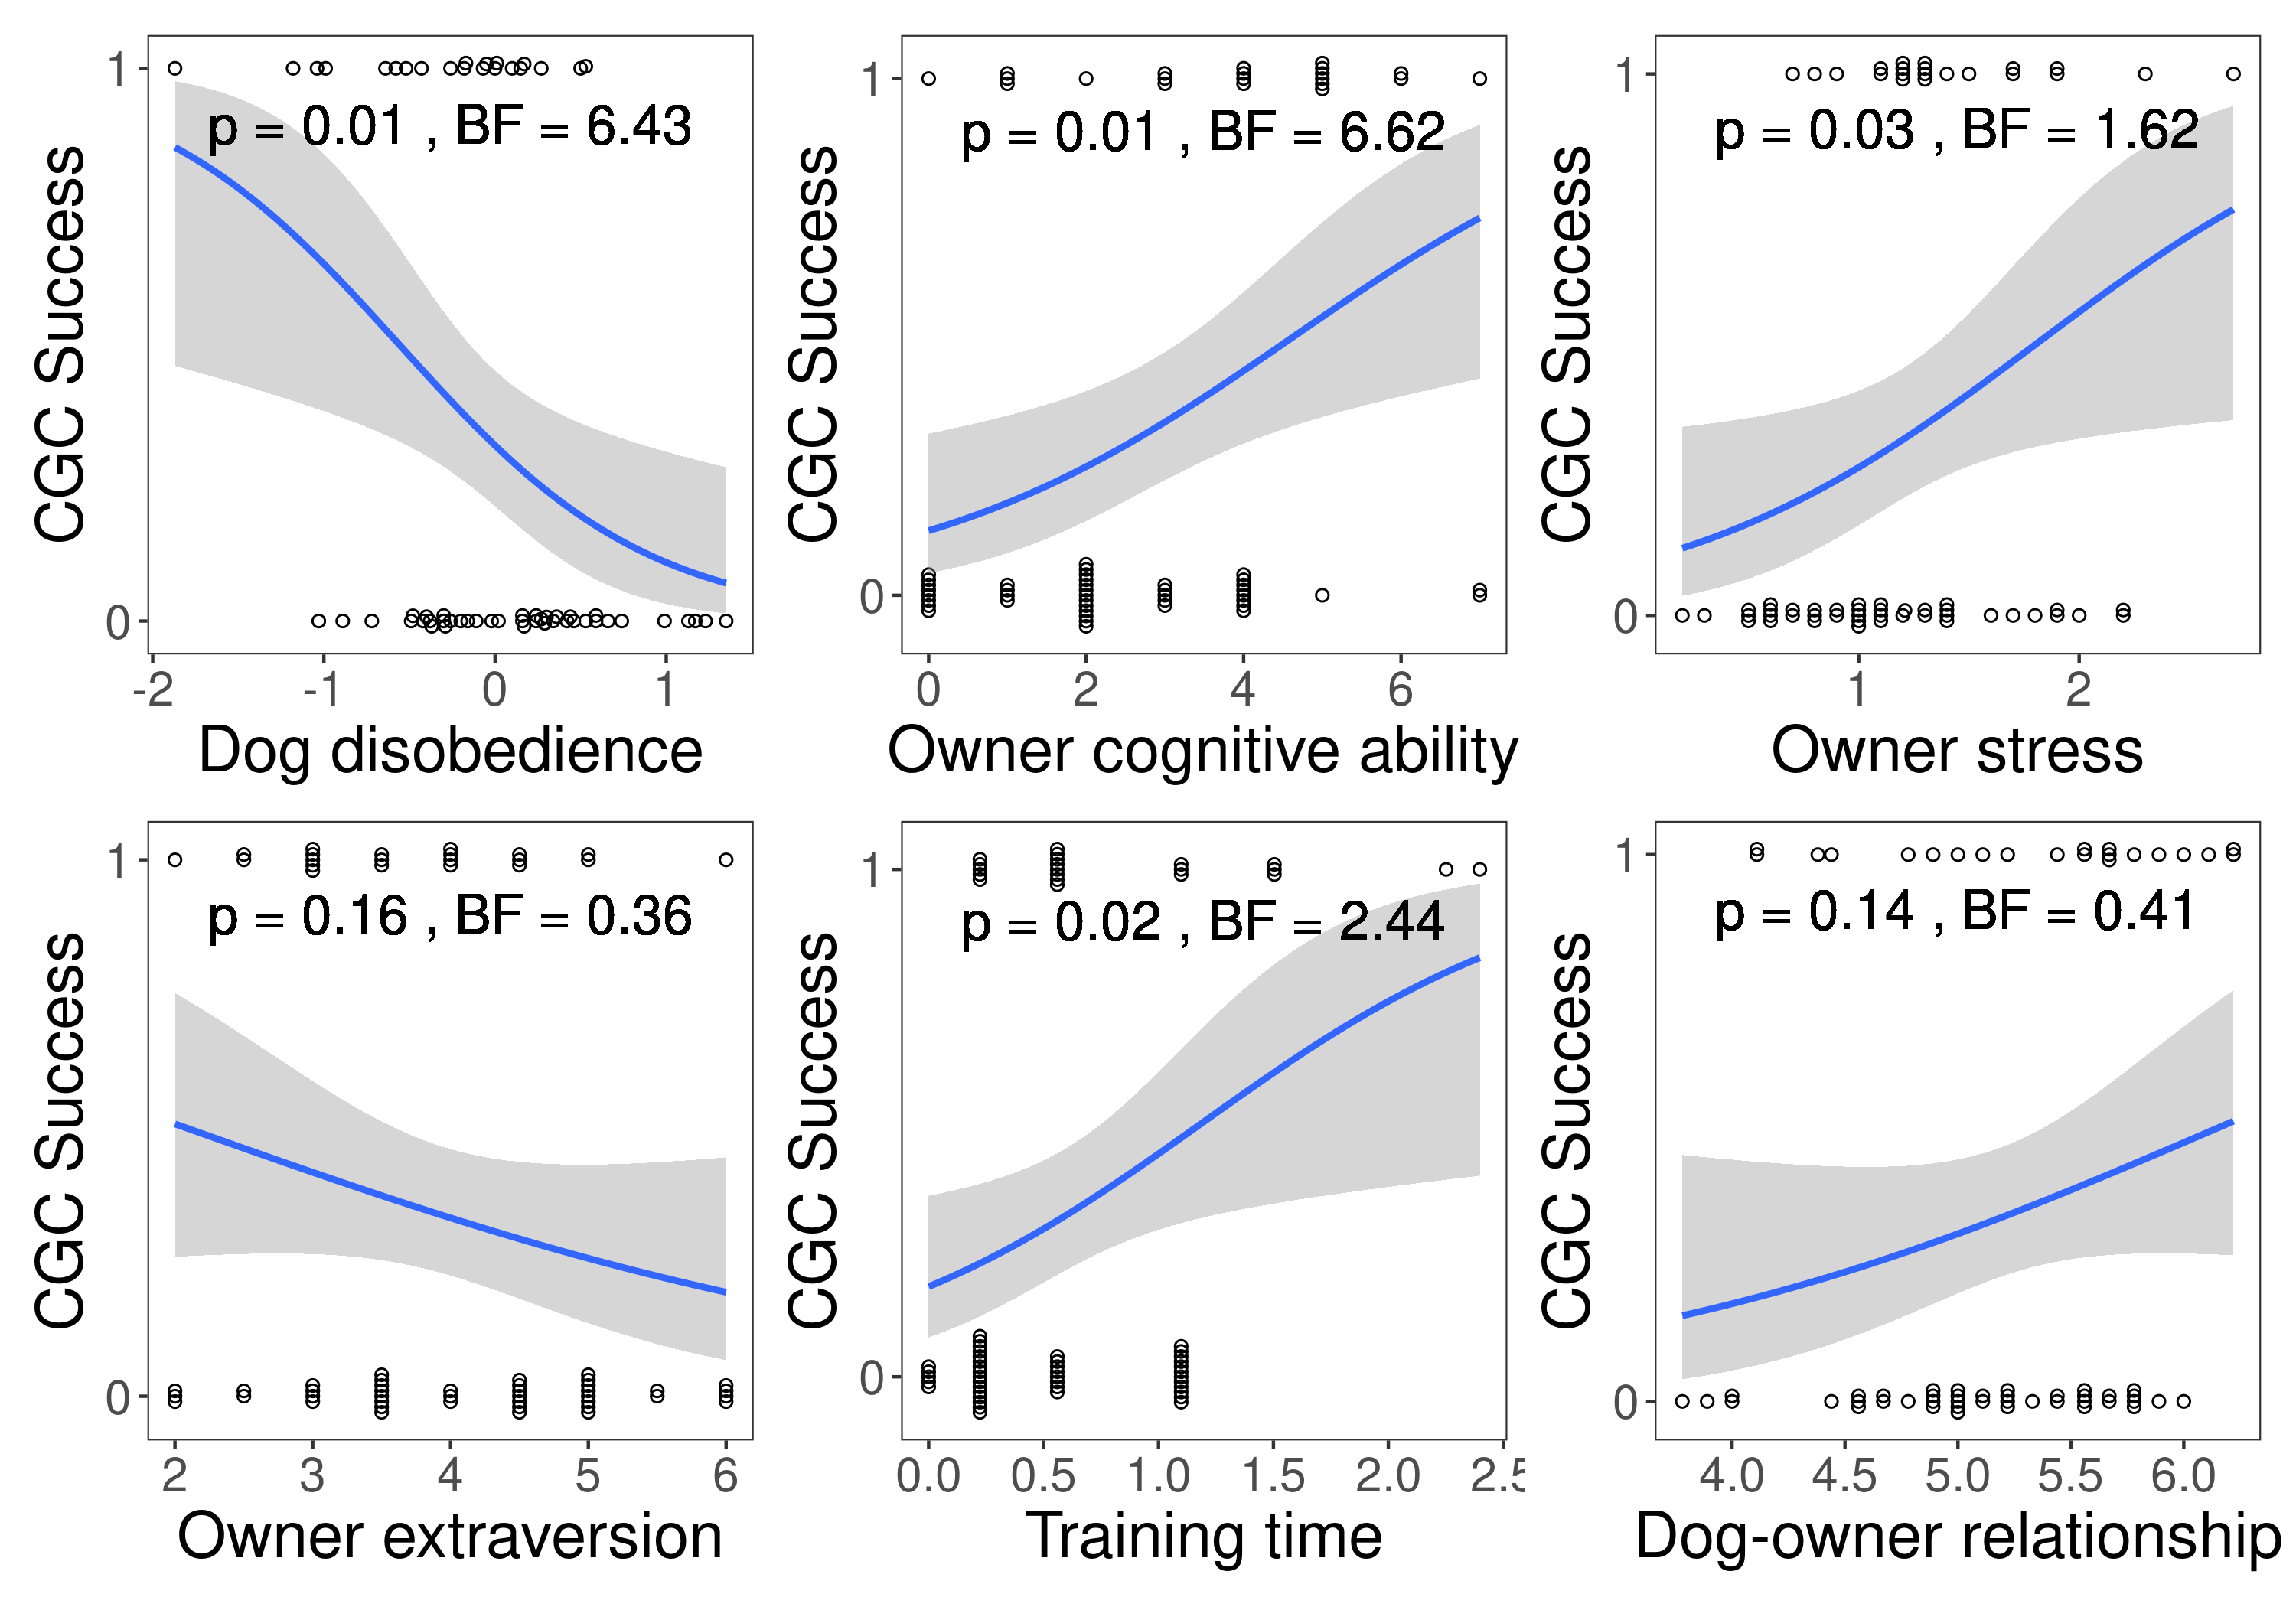
\includegraphics[width=1\linewidth]{/media/jstevens/data/jstevens/OneDrive/active_sync/projects/dogobedience2021/figures/cgc_plots} \caption{Effects of predictors on Canine Good Citizen training success. We conducted logistic regression analyses for each predictor. Open circles represent individual data points, curves represented fitted logistic regression lines, and the bands represent 95\% confidence intervals for regression curves.}\label{fig:cgc-predictors}
\end{figure*}

Though multiple regression is the standard model for investigating factors that influence response variables, we also used machine-learning techniques to further explore these factors. We had four machine-learning algorithms and logistic regression predict training success using the six predictors from the pairwise analysis. First, we examined the predictive accuracy of the models and found considerable differences across models (Figure S2), with C5.0 producing the highest accuracy (83.2±2.9\%). Logistic regression (74.8±3.0\%), random forest (75.0±2.9\%), and neural networks (74.2±3.6\%) yielded intermediate accuracy and CART (67.9±3.5\%) performed worst.

With the regression and machine-learning models, we can calculate predictor importance, which offers a continuous measure of the contribution of each predictor to the predictive accuracy of the models. Figure \ref{fig:cgc-predictor-imp} shows the mean importance of each predictor for the Canine Good Citizen training success as well as predictor importance for each model. When aggregating across the models, owner cognitive ability is the most important predictor of training success. Dog disobedience was the second most important predictor, followed by training time. Some machine-learning algorithms found important predictors that regression did not favor (e.g., training time), and regression favored predictors not strongly favored by all algorithms (e.g., owner stress).



\begin{figure*}
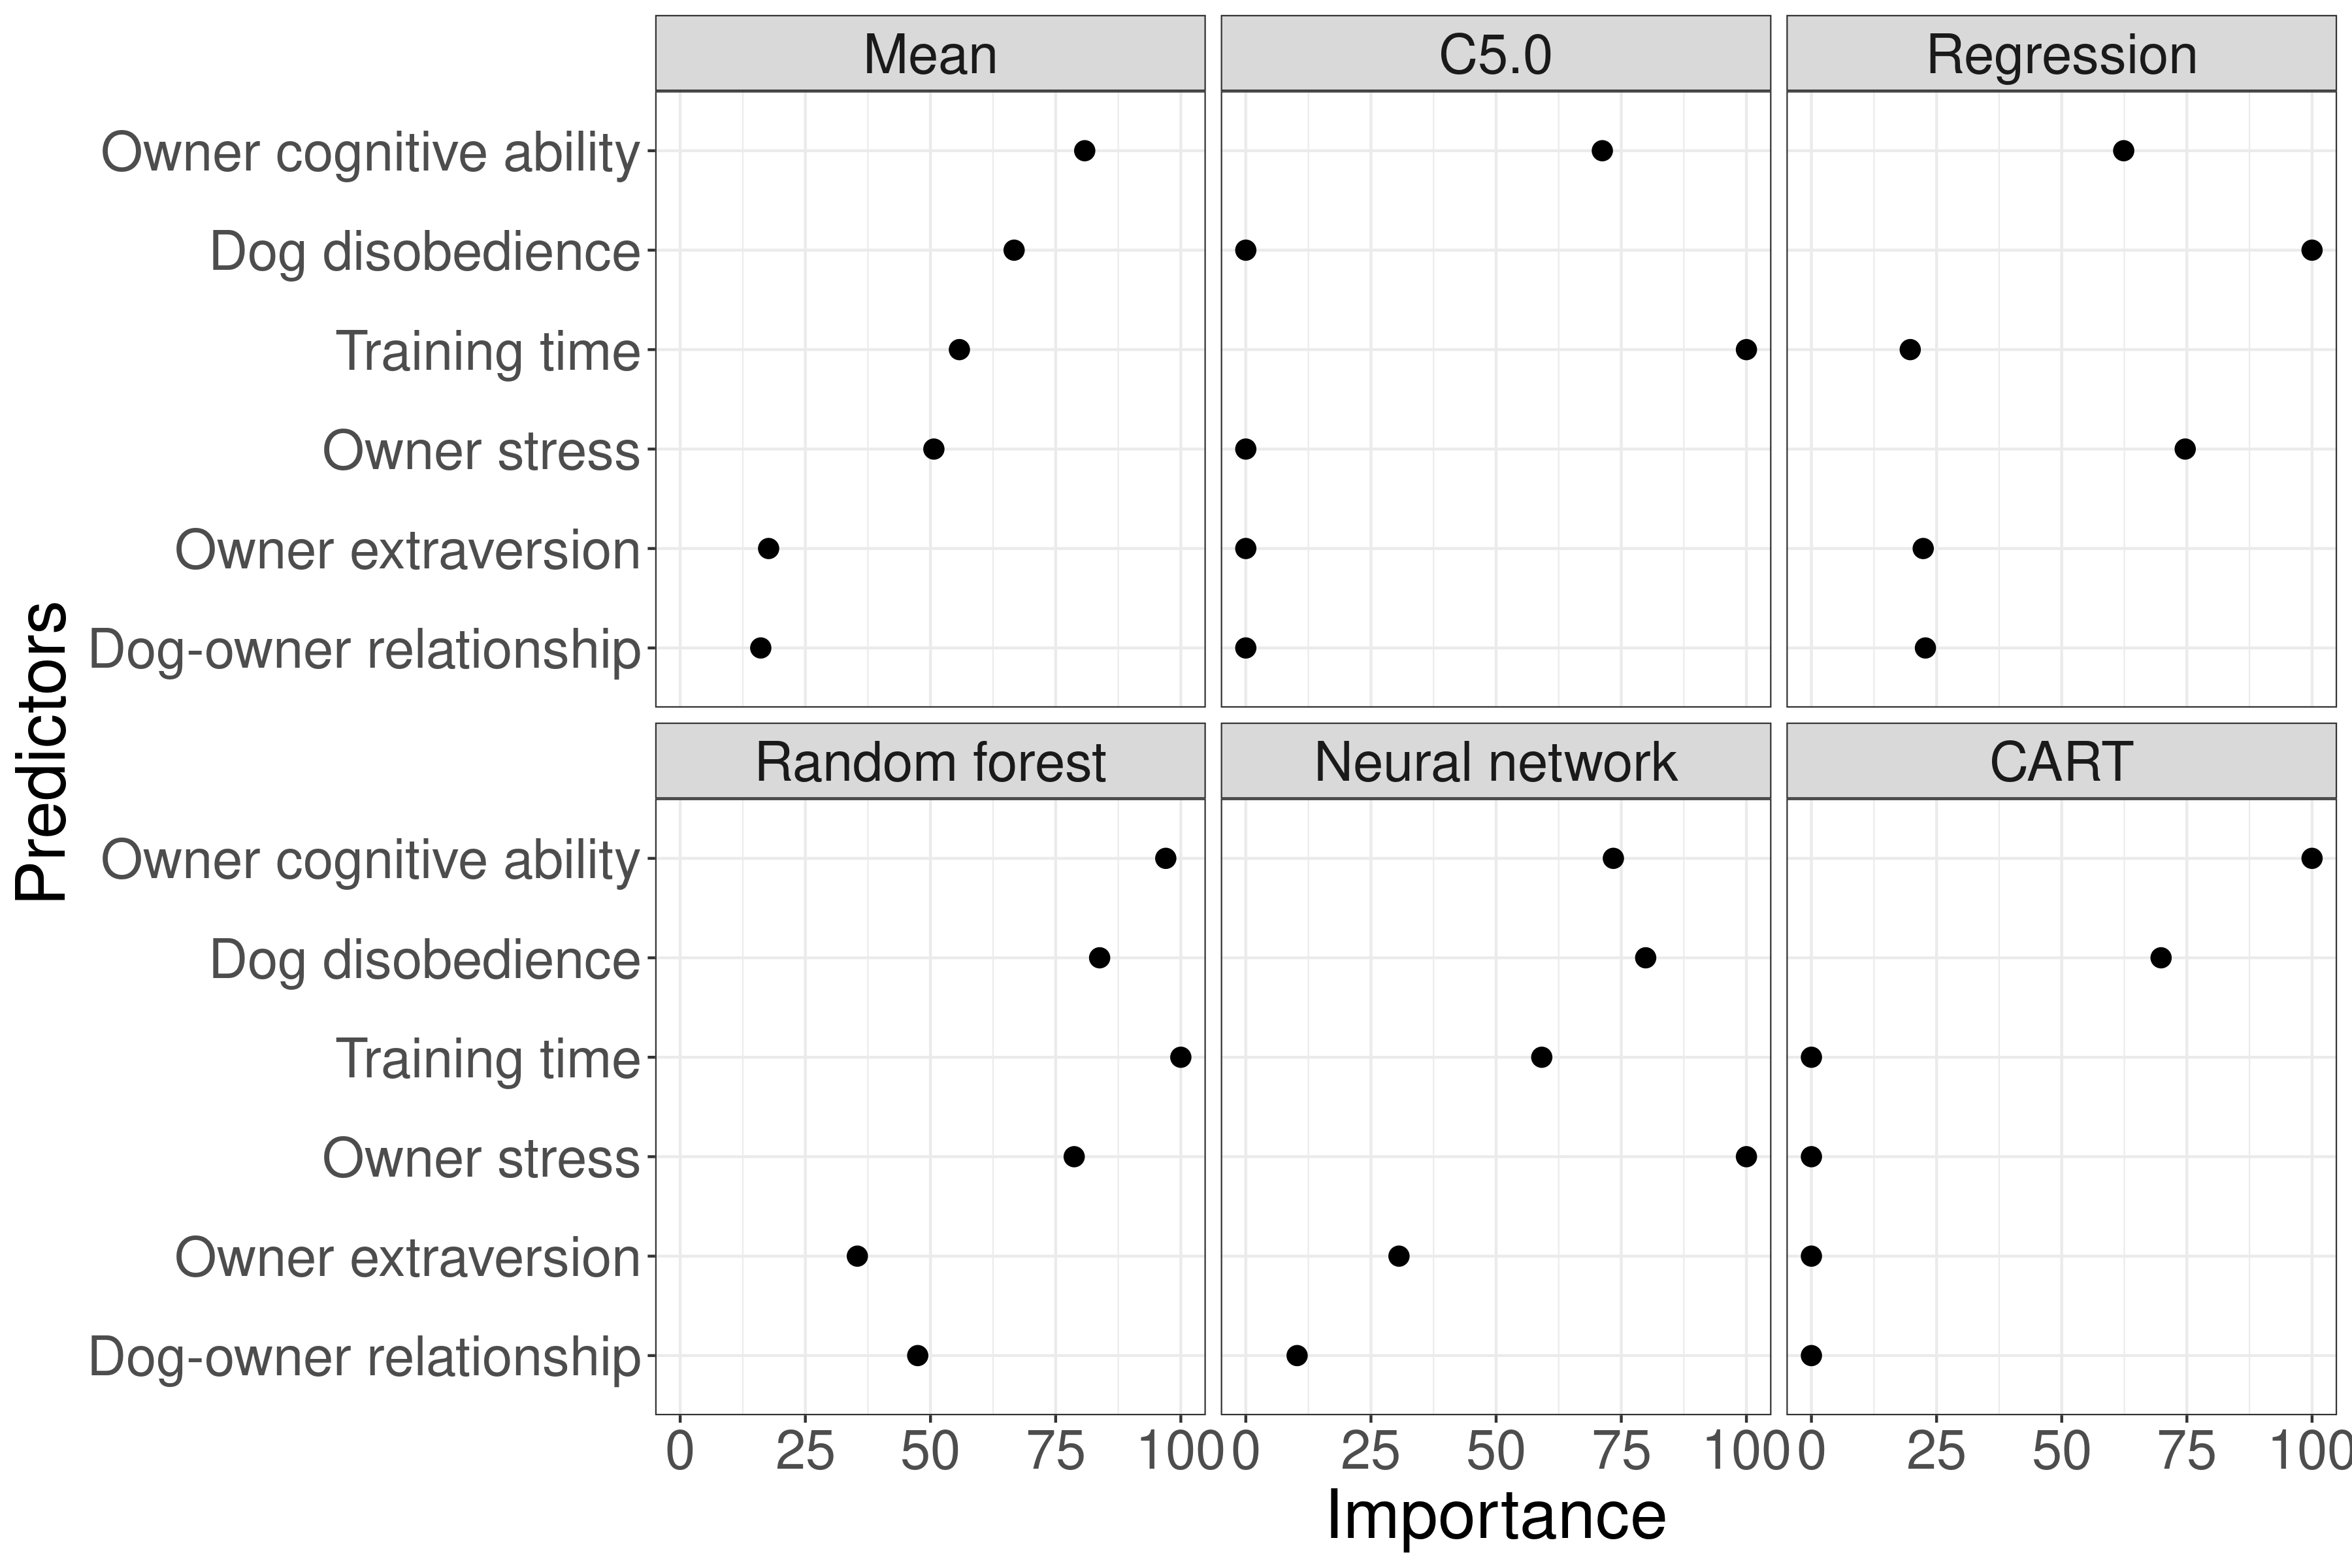
\includegraphics[width=1\linewidth]{/media/jstevens/data/jstevens/OneDrive/active_sync/projects/dogobedience2021/figures/cgc_predictor_importance_algorithm} \caption{Predictor importance for Canine Good Citizen training success. The first panel represents the mean importance over all predictors (predictors ordered by mean importance). The remaining panels show importance for each predictor (panels ordered by predictor accuracy). Closed circles represent importance scores for each model and predictor.}\label{fig:cgc-predictor-imp}
\end{figure*}

\hypertarget{discussion}{%
\section{Discussion}\label{discussion}}

Using logistic regression models and machine-learning algorithms, we found that characteristics of the dog (low levels of disobedience), the owner (high levels of certain cognitive abilities), and dog-owner interactions (more time spent training) were all important in predicting Canine Good Citizen training success. In terms of dog characteristics, disobedience (Bennett \& Rohlf's (2007) disobedience subscale) predicted passing the test. This is perhaps not surprising as the Canine Good Citizen test focuses on simple obedience behaviors including sit, down, and stay. The Bennett \& Rohlf disobedience subscale asks about good manners, sit, stay, come, and soiling in the house. Demographic information about the dog, including sex, age, and neuter status did not predict training success.

We found no strong predictive power of any owner personality dimensions. Surprisingly, the diligence required to consistently and successfully train a dog was not captured in the owner personality trait of conscientiousness. Also, neuroticism---a trait linked to command-following (Kis et al., 2012)---was not related to training success. Perhaps the brief personality scale used here did not provide the most reliable measure of owner personality.

One of the strongest owner characteristics that predicted training success was cognitive ability. We combined the scores from two tests of cognitive ability: the Cognitive Reflection Test and the Berlin Numeracy Test. The Cognitive Reflection Test (Frederick, 2005) assesses the cognitive flexibility to inhibit falling for an obvious but incorrect solution to a problem instead reflecting deeply to find the correct solution. Cognitive reflection is associated with high-level reasoning, reduced cognitive biases, and superior decision making (Sobkow et al., 2020). The Berlin Numeracy Test assesses understanding and processing of probabilistic and statistical information, and it is crucial for interpreting risk and superior decision making (Cokely et al., 2012; Skagerlund et al., 2018). Both measures capture cognitive performance above and beyond traditional measures of cognitive ability (Sobkow et al., 2020). We combined these two measures additively and found it to be one of the strongest predictors of training success potentially due to enhanced decision making. Owner cognitive ability may have a direct effect on training success by owners high in these certain aspects of cognitive ability making better decisions about selecting dogs that are likely to succeed in the test. They may research and select breed types or specific breeders that tend to have well-behaved or easily trainable dogs. If they adopt dogs, they may take more time to observe the dog's behavior or simply be better at selecting trainable dogs. Alternatively, the higher cognitive abilities may not directly result in training success. Instead, these cognitive abilities may be correlated with other characteristics that have more of a direct influence on training success. For instance, high cognitive ability owners may foresee the value of a well-trained dog and be more consistent and exert more time and effort in their training than lower cognitive ability owners. Relatedly, the cognitive ability scores may capture the participants' amount of effort exerted on the survey (rather than actual cognitive ability), which could also relate to the effort that they are willing to invest in training. Unfortunately, we do not have a measure of training time during the training class, but we would predict that cognitive ability would correlate with training effort, which, in turn, would predict training success. This result, however, was not predicted based on a theoretically driven framework. Thus, this exploratory result must be replicated to validate the findings.

Finally, we consider dog-owner interactions, that is, characteristics that require both dog and owner. The quality of the dog-human relationship is an important characteristic that is related to many important components such as dog cognitive performance (Topál et al., 1997), dog quality of life (Marinelli et al., 2007), ownership satisfaction (Herwijnen et al., 2018), and some elements of dog training such as class attendance and type of training aid (Herwijnen et al., 2018). Though dog-owner relationship quality was included in the potential predictors for our study, it ranked second to last in terms of predictor importance, suggesting it did not strongly predict training success. However, other dog-owner interactions were important predictors: amount of time spent training the dog before the first class period. Dogs whose owners spent more time training their dog \emph{before the course started} were more likely to pass the test. Again, training before the class began likely resulted in more time spent training during course, which would increase the likelihood of passing the test. This finding suggests that exposing dogs to training before formal classes could go a long way to improving their training success.

For this analysis, we combined dogs who failed the Canine Good Citizen test with those who did not take the test as our unsuccessful training outcome. While ideally we would exclude dogs who did not take the test, only 3 dogs failed the test, which did not provide enough unsuccessful responses to properly analyze our data. We combined these two outcomes for this analysis because it is likely that some owners did not take the test because their dogs were not trained sufficiently to pass the test. However, owners may have avoided the test for other reasons, including they dropped out of the course, their dogs were not quite prepared for the test, or their schedule did not allow it. Therefore, we should interpret these results cautiously, and further larger-scale studies should replicate these methods to confirm the findings.

As a note of caution, this study only included the training success of dog/owner pairs who took a single trainer's class and were evaluated by a single examiner. Trainers likely vary dramatically in the philosophies and techniques used to teach owners how to work with their dogs (Feng et al., 2018). Also, examiners likely vary in the criteria used to establish test success. Our sample of dog owners were primarily female (57 of 62 owners were female), which could potentially bias our results. Further, our sample of dogs and owners may be biased due to the self-selection of volunteers. This variability coupled with the exploratory nature of this study suggests that we should be cautious about generalizing these findings beyond the study sample, and further work should attempt to replicate the findings. The Canine Good Citizen program, however, can provide some degree of standardization in terms of a consistent measure of training. Given the large number of dogs participating in the program, this offers an interesting avenue for future research on dog training.

\hypertarget{machine-learning}{%
\subsection{Machine learning}\label{machine-learning}}

Machine learning is a powerful set of tools that can apply across a wide range of data (Hastie et al., 2009; Kuhn \& Johnson, 2013). While it is commonly used in other fields, comparative psychology has been slow to pick up machine-learning methods, though they have been introduced in the field of animal behavior more generally (Valletta et al., 2017). Our field has traditionally relied on various forms of linear models (Lindeløv, 2019) for our statistical analyses.

Machine learning opens up new ways of thinking about our data analysis. For instance, machine learning highlights the notion of prediction over explanation (Yarkoni \& Westfall, 2017). That is, most psychological studies attempt to explain patterns of data by fitting statistical models to them. However, often we really want to predict new data---we want to see if our models generalize beyond the data that we collected. Machine-learning approaches do this by training models to a subset of the data, fixing the parameters of the models based on the training data, using the trained models to predict new data, and measuring how well the trained models predict the test data. One key benefit to prediction over fitting is that it reduces bias in our conclusions (Brighton \& Gigerenzer, 2015). Typically, though, we do not have very large data sets, so the training and testing subsets may be rather small, thus creating a lot of variance. To reduce the variance, we can use cross-validation, where we repeatedly partition the data into training and testing subsets, fit the models, predict new data, and calculate a mean predictive accuracy over all of the repetitions (de Rooij \& Weeda, 2020). Therefore, we reduce bias error by predicting new data and variance error by repeatedly sampling from our data.

Of course, prediction and cross-validation can be used with regression models as well as machine-learning algorithms (de Rooij \& Weeda, 2020). So does machine learning offer more than regression? Our results suggest that it can. Because machine-learning models use completely different methods for classifying responses compared to regression, they can generate completely different results, which provides two benefits. First, machine-learning algorithms can predict responses better than regression. For example, we found that the decision-tree algorithm C5.0 dramatically outpredicted regression for Canine Good Citizen training success. If model prediction accuracy is important, some machine-learning models may outperform regression. Second, different methods in machine-learning models can allow them to discover distinct predictors that regression may overlook. By using exclusively regression analyses, we are limiting our understanding of the relationship between predictors and responses by focusing on a single set of assumptions and analytical techniques. Machine learning breaks us out of the constraints imposed by regression. This can be important in both confirming existing theories and developing new hypotheses.

There can be drawbacks to machine-learning approaches, however (Adjerid \& Kelley, 2018; Jacobucci \& Grimm, 2020). Unlike linear models, many core machine-learning algorithms cannot handle missing data. Therefore, researchers must discard cases with missing data or impute missing values. It is likely that both of these strategies can bias results. Also, some machine-learning algorithms (along with linear models) perform poorly if predictors are highly correlated, or multicollinear (Kuhn \& Johnson, 2013). So some predictors need to be removed to minimize this. Further, some models do not perform well with large number of predictors, so filters must be used to remove extra predictors (Kuhn \& Johnson, 2019). We used a simple filter based on regression analyses, so our results could have been different if we did not use that filter. Finally, there are many machine-learning algorithms available, so it can be difficult to choose which algorithms to include in the analysis. Fortunately, there are a number of core algorithms that are used frequently and are well-understood mathematically (Hastie et al., 2009; Valletta et al., 2017). Because of their usefulness and common use, they are relatively easy to implement in statistical packages such as R (R Core Team, 2020) and JASP (JASP Team, 2020).

\hypertarget{conclusion}{%
\subsection{Conclusion}\label{conclusion}}

In the present study, we conducted an exploration of dog, owner, and dog-owner characteristics that predict training success. We found that certain aspects of owner cognitive ability, dog disobedience, and time spent training were the most important factors in predicting training success. Therefore, dog, owner, and dog-owner characteristics were all important for completion of the Canine Good Citizen training program. Though dogs with owner-perceived problem behaviors and disobedience issues struggle, owners who put forth time, energy, and effort towards their goals are most likely to succeed in training. Assessing characteristics of dogs and owners can provide important insights into potential interventions and training techniques that may cater to the specific characteristics of dog-owner pairs for pet dogs and potentially working dogs.

\hypertarget{acknowledgments}{%
\section{Acknowledgments}\label{acknowledgments}}

This research was funded by a University of Nebraska-Lincoln College of Arts and Sciences Partnership Seed Grant. We would like to thank Kylie Hughes, Elise Thayer, Toria Biancalana, and McKenna Yohe for collecting saliva samples, Tierney Lorenz for her expertise on dog saliva collection, Jessica Calvi and the University of Nebraska-Lincoln Salivary Bioscience Laboratory for assaying saliva samples, and Billy Lim for comments on an early draft.

\hypertarget{declarations}{%
\section{Declarations}\label{declarations}}

\hypertarget{funding}{%
\subsection{Funding}\label{funding}}

This research was funded by a University of Nebraska-Lincoln College of Arts and Sciences Partnership Seed Grant.

\hypertarget{conflicts-of-interest}{%
\subsection{Conflicts of interest}\label{conflicts-of-interest}}

JRS and his dog completed one of the Prairie Skies Dog Training courses in this study starting with the second class session. He did not complete any of the surveys or behavioral tasks, so he has no data included in this analysis. JRS received donations for research and outreach activities from Prairie Skies Dog Training (owned by JM), Arnie's Pet Food Store, Green Spot, Kenl Inn, Nature's Logic, Nature's Variety, Nebraska Animal Medical Center, Norland Pure, Pepsi, Raising Cane's, Sirius Veterinary Orthopedic Center, Smarty Dog Training, Stubbs Chiropractic, and private donors. JM is the owner of Prairie Skies Dog Training and received payments for training services from the participants in this study.

\hypertarget{ethics-approval}{%
\subsection{Ethics approval}\label{ethics-approval}}

All procedures were conducted in an ethical and responsible manner, in full compliance with all relevant codes of experimentation and legislation and were approved by the UNL Internal Review Board (protocol \# 17922) and Institutional Animal Care and Use Committee (protocol \# 1621).

\hypertarget{consent-to-participate-and-for-publication}{%
\subsection{Consent to participate and for publication}\label{consent-to-participate-and-for-publication}}

All participants offered consent to participate, and they acknowledged that de-identified data could be published publicly.

\hypertarget{availability-of-data-and-material}{%
\subsection{Availability of data and material}\label{availability-of-data-and-material}}

All data files, data analysis scripts, and supplementary materials (surveys, tables, figures) are available at \url{https://osf.io/3p5vx/}.

\hypertarget{authors-contributions}{%
\subsection{Authors' contributions}\label{authors-contributions}}

The authors made the following contributions. Jeffrey R. Stevens: Conceptualization, Data Curation, Formal Analysis, Funding Acquisition, Investigation, Methodology, Project Administration, Resources, Software, Supervision, Visualization, Writing - Original Draft Preparation, Writing - Review \& Editing;
London M. Wolff: Formal Analysis, Investigation, Methodology, Writing - Original Draft Preparation, Writing - Review \& Editing;
Megan Bosworth: Investigation, Methodology, Writing - Review \& Editing;
Jill Morstad: Conceptualization, Resources, Writing - Review \& Editing.

\hypertarget{references}{%
\section*{References}\label{references}}
\addcontentsline{toc}{section}{References}

\hypertarget{refs}{}
\begin{CSLReferences}{1}{0}
\leavevmode\hypertarget{ref-Adjerid.Kelley.2018}{}%
Adjerid, I., \& Kelley, K. (2018). Big data in psychology: {A} framework for research advancement. \emph{American Psychologist}, \emph{73}(7), 899--917. \url{https://doi.org/10.1037/amp0000190}

\leavevmode\hypertarget{ref-Arhant.etal.2010}{}%
Arhant, C., Bubna-Littitz, H., Bartels, A., Futschik, A., \& Troxler, J. (2010). Behaviour of smaller and larger dogs: {Effects} of training methods, inconsistency of owner behaviour and level of engagement in activities with the dog. \emph{Applied Animal Behaviour Science}, \emph{123}(3), 131--142. \url{https://doi.org/10.1016/j.applanim.2010.01.003}

\leavevmode\hypertarget{ref-R-papaja}{}%
Aust, F., \& Barth, M. (2020). \emph{{papaja}: {Create} {APA} manuscripts with {R Markdown}}. \url{https://github.com/crsh/papaja}

\leavevmode\hypertarget{ref-R-lme4}{}%
Bates, D., Mächler, M., Bolker, B., \& Walker, S. (2015). Fitting linear mixed-effects models using {lme4}. \emph{Journal of Statistical Software}, \emph{67}(1), 1--48. \url{https://doi.org/10.18637/jss.v067.i01}

\leavevmode\hypertarget{ref-Bennett.Rohlf.2007}{}%
Bennett, P. C., \& Rohlf, V. I. (2007). Owner-companion dog interactions: {Relationships} between demographic variables, potentially problematic behaviours, training engagement and shared activities. \emph{Applied Animal Behaviour Science}, \emph{102}(1), 65--84. \url{https://doi.org/10.1016/j.applanim.2006.03.009}

\leavevmode\hypertarget{ref-Breiman.2001a}{}%
Breiman, L. (2001). Random forests. \emph{Machine Learning}, \emph{45}(1), 5--32. \url{https://doi.org/10.1023/A:1010933404324}

\leavevmode\hypertarget{ref-Breiman.etal.1984}{}%
Breiman, L., Friedman, J. H., Olshen, R. A., \& Stone, C. J. (1984). \emph{Classification and {Regression Trees}}. {Chapman and Hall}.

\leavevmode\hypertarget{ref-Brighton.Gigerenzer.2015}{}%
Brighton, H., \& Gigerenzer, G. (2015). The bias bias. \emph{Journal of Business Research}, \emph{68}(8), 1772--1784. \url{https://doi.org/10.1016/j.jbusres.2015.01.061}

\leavevmode\hypertarget{ref-Cavanaugh.etal.2008}{}%
Cavanaugh, L. A., Leonard, H. A., \& Scammon, D. L. (2008). A tail of two personalities: {How} canine companions shape relationships and well-being. \emph{Journal of Business Research}, \emph{61}(5), 469--479. \url{https://doi.org/10.1016/j.jbusres.2007.07.024}

\leavevmode\hypertarget{ref-Chopik.Weaver.2019}{}%
Chopik, W. J., \& Weaver, J. R. (2019). Old dog, new tricks: {Age} differences in dog personality traits, associations with human personality traits, and links to important outcomes. \emph{Journal of Research in Personality}, \emph{79}, 94--108. \url{https://doi.org/10.1016/j.jrp.2019.01.005}

\leavevmode\hypertarget{ref-Clark.Boyer.1993}{}%
Clark, G. I., \& Boyer, W. N. (1993). The effects of dog obedience training and behavioural counselling upon the human-canine relationship. \emph{Applied Animal Behaviour Science}, \emph{37}(2), 147--159. \url{https://doi.org/10.1016/0168-1591(93)90107-Z}

\leavevmode\hypertarget{ref-R-ggbeeswarm}{}%
Clarke, E., \& Sherrill-Mix, S. (2017). \emph{Ggbeeswarm: Categorical scatter (violin point) plots}. \url{https://CRAN.R-project.org/package=ggbeeswarm}

\leavevmode\hypertarget{ref-Cobb.etal.2016}{}%
Cobb, M. L., Iskandarani, K., Chinchilli, V. M., \& Dreschel, N. A. (2016). A systematic review and meta-analysis of salivary cortisol measurement in domestic canines. \emph{Domestic Animal Endocrinology}, \emph{57}, 31--42. \url{https://doi.org/10.1016/j.domaniend.2016.04.003}

\leavevmode\hypertarget{ref-Cohen.etal.1983}{}%
Cohen, S., Kamarck, T., \& Mermelstein, R. (1983). A global measure of perceived stress. \emph{Journal of Health and Social Behavior}, \emph{24}(4), 385--396. \url{https://doi.org/10.2307/2136404}

\leavevmode\hypertarget{ref-Cokely.etal.2012}{}%
Cokely, E. T., Galesic, M., Schulz, E., Ghazal, S., \& Garcia-Retamero, R. (2012). Measuring risk literacy: {The Berlin Numeracy Test}. \emph{Judgment and Decision Making}, \emph{7}(1), 25--47.

\leavevmode\hypertarget{ref-Curb.etal.2013}{}%
Curb, L. A., Abramson, C. I., Grice, J. W., \& Kennison, S. M. (2013). The relationship between personality match and pet satisfaction among dog owners. \emph{Anthrozoös}, \emph{26}(3), 395--404. \url{https://doi.org/10.2752/175303713X13697429463673}

\leavevmode\hypertarget{ref-Daye.2011}{}%
Daye, M. (2011). \emph{Dog owner personality, owner interaction with dog, and dog aggression} {[}Ph.\{\{D\}\}. Thesis{]}. Alliant International University.

\leavevmode\hypertarget{ref-deRooij.Weeda.2020}{}%
de Rooij, M., \& Weeda, W. (2020). Cross-validation: {A} method every psychologist should know. \emph{Advances in Methods and Practices in Psychological Science}, \emph{3}(2), 248--263. \url{https://doi.org/10.1177/2515245919898466}

\leavevmode\hypertarget{ref-Dodman.etal.2018}{}%
Dodman, N. H., Brown, D. C., \& Serpell, J. A. (2018). Associations between owner personality and psychological status and the prevalence of canine behavior problems. \emph{PLOS ONE}, \emph{13}(2), e0192846. \url{https://doi.org/10.1371/journal.pone.0192846}

\leavevmode\hypertarget{ref-Dreschel.Granger.2009}{}%
Dreschel, N. A., \& Granger, D. A. (2009). Methods of collection for salivary cortisol measurement in dogs. \emph{Hormones and Behavior}, \emph{55}(1), 163--168. \url{https://doi.org/10.1016/j.yhbeh.2008.09.010}

\leavevmode\hypertarget{ref-Dwyer.etal.2006}{}%
Dwyer, F., Bennett, P. C., \& Coleman, G. J. (2006). Development of the {Monash Dog Owner Relationship Scale} ({MDORS}). \emph{Anthrozoös}, \emph{19}(3), 243--256. \url{https://doi.org/10.2752/089279306785415592}

\leavevmode\hypertarget{ref-Feng.etal.2018}{}%
Feng, L. C., Howell, T. J., \& Bennett, P. C. (2018). Practices and perceptions of clicker use in dog training: {A} survey-based investigation of dog owners and industry professionals. \emph{Journal of Veterinary Behavior}, \emph{23}, 1--9. \url{https://doi.org/10.1016/j.jveb.2017.10.002}

\leavevmode\hypertarget{ref-Frederick.2005}{}%
Frederick, S. (2005). Cognitive reflection and decision making. \emph{Journal of Economic Perspectives}, \emph{19}(4), 25--42. \url{https://doi.org/10.1257/089533005775196732}

\leavevmode\hypertarget{ref-Furnkranz.2010}{}%
Fürnkranz, J. (2010). Decision tree. In C. Sammut \& G. I. Webb (Eds.), \emph{Encyclopedia of {Machine Learning}} (pp. 263--267). {Springer}. \url{https://doi.org/10.1007/978-0-387-30164-8_204}

\leavevmode\hypertarget{ref-Gosling.etal.2003}{}%
Gosling, S. D., Rentfrow, P. J., \& Swann, W. B. (2003). A very brief measure of the {Big}-{Five} personality domains. \emph{Journal of Research in Personality}, \emph{37}(6), 504--528. \url{https://doi.org/10.1016/S0092-6566(03)00046-1}

\leavevmode\hypertarget{ref-R-vip}{}%
Greenwell, B. M., \& Boehmke, B. C. (2020). Variable importance plots---an introduction to the vip package. \emph{The R Journal}, \emph{12}(1), 343--366. \url{https://doi.org/10.32614/RJ-2020-013}

\leavevmode\hypertarget{ref-Hastie.etal.2009}{}%
Hastie, T., Tibshirani, R., \& Friedman, J. H. (2009). \emph{The {Elements} of {Statistical Learning}: {Data Mining}, {Inference}, and {Prediction}}. {Springer}.

\leavevmode\hypertarget{ref-Herwijnen.etal.2018}{}%
Herwijnen, I. R. van, Borg, J. A. M. van der, Naguib, M., \& Beerda, B. (2018). Dog ownership satisfaction determinants in the owner-dog relationship and the dog's behaviour. \emph{PLOS ONE}, \emph{13}(9), e0204592. \url{https://doi.org/10.1371/journal.pone.0204592}

\leavevmode\hypertarget{ref-Hiby.etal.2004}{}%
Hiby, E., Rooney, N., \& Bradshaw, J. (2004). Dog training methods: Their use, effectiveness and interaction with behaviour and welfare. \emph{Animal Welfare}, \emph{13}(1), 63--69.

\leavevmode\hypertarget{ref-Hsu.Serpell.2003}{}%
Hsu, Y., \& Serpell, J. A. (2003). Development and validation of a questionnaire for measuring behavior and temperament traits in pet dogs. \emph{Journal of the American Veterinary Medical Association}, \emph{223}(9), 1293--1300. \url{https://doi.org/10.2460/javma.2003.223.1293}

\leavevmode\hypertarget{ref-Jacobucci.Grimm.2020}{}%
Jacobucci, R., \& Grimm, K. J. (2020). Machine learning and psychological research: {The} unexplored effect of measurement. \emph{Perspect Psychol Sci}, \emph{15}(3), 809--816. \url{https://doi.org/10.1177/1745691620902467}

\leavevmode\hypertarget{ref-Jagoe.Serpell.1996}{}%
Jagoe, A., \& Serpell, J. (1996). Owner characteristics and interactions and the prevalence of canine behaviour problems. \emph{Applied Animal Behaviour Science}, \emph{47}(1), 31--42. \url{https://doi.org/10.1016/0168-1591(95)01008-4}

\leavevmode\hypertarget{ref-JASPTeam.2020}{}%
JASP Team. (2020). \emph{{JASP} (version 0.13.12){[}{Computer} software{]}}.

\leavevmode\hypertarget{ref-R-ggcorrplot}{}%
Kassambara, A. (2019). \emph{Ggcorrplot: Visualization of a correlation matrix using 'ggplot2'}. \url{https://CRAN.R-project.org/package=ggcorrplot}

\leavevmode\hypertarget{ref-Kis.etal.2012}{}%
Kis, A., Turcsán, B., Miklósi, Á., \& Gácsi, M. (2012). The effect of the owner's personality on the behaviour of owner-dog dyads. \emph{Interaction Studies}, \emph{13}(3), 373--385. \url{https://doi.org/10.1075/is.13.3.03kis}

\leavevmode\hypertarget{ref-Kobelt.etal.2003a}{}%
Kobelt, A. J., Hemsworth, P. H., Barnett, J. L., \& Coleman, G. J. (2003). A survey of dog ownership in suburban {Australia}---conditions and behaviour problems. \emph{Applied Animal Behaviour Science}, \emph{82}(2), 137--148. \url{https://doi.org/10.1016/S0168-1591(03)00062-5}

\leavevmode\hypertarget{ref-Konok.etal.2015}{}%
Konok, V., Kosztolányi, A., Rainer, W., Mutschler, B., Halsband, U., \& Miklósi, Á. (2015). Influence of owners' attachment style and personality on their dogs' ({Canis} familiaris) separation-related disorder. \emph{PLOS ONE}, \emph{10}(2), e0118375. \url{https://doi.org/10.1371/journal.pone.0118375}

\leavevmode\hypertarget{ref-Koo.Li.2016}{}%
Koo, T. K., \& Li, M. Y. (2016). A guideline of selecting and reporting intraclass correlation coefficients for reliability research. \emph{Journal of Chiropractic Medicine}, \emph{15}(2), 155--163. \url{https://doi.org/10.1016/j.jcm.2016.02.012}

\leavevmode\hypertarget{ref-Kubinyi.etal.2009}{}%
Kubinyi, E., Turcsán, B., \& Miklósi, Á. (2009). Dog and owner demographic characteristics and dog personality trait associations. \emph{Behavioural Processes}, \emph{81}(3), 392--401. \url{https://doi.org/10.1016/j.beproc.2009.04.004}

\leavevmode\hypertarget{ref-R-caret}{}%
Kuhn, M. (2020). \emph{Caret: Classification and regression training}. \url{https://CRAN.R-project.org/package=caret}

\leavevmode\hypertarget{ref-Kuhn.Johnson.2019}{}%
Kuhn, M., \& Johnson, K. (2019). \emph{Feature {Engineering} and {Selection}: {A Practical Approach} for {Predictive Models}}. {CRC Press}.

\leavevmode\hypertarget{ref-Kuhn.Johnson.2013}{}%
Kuhn, M., \& Johnson, K. (2013). \emph{Applied {Predictive Modeling}}. {Springer}.

\leavevmode\hypertarget{ref-R-C50}{}%
Kuhn, M., \& Quinlan, R. (2020). \emph{C50: C5.0 decision trees and rule-based models}. \url{https://CRAN.R-project.org/package=C50}

\leavevmode\hypertarget{ref-R-tidymodels}{}%
Kuhn, M., \& Wickham, H. (2020). \emph{Tidymodels: A collection of packages for modeling and machine learning using tidyverse principles.} \url{https://www.tidymodels.org}

\leavevmode\hypertarget{ref-Kwan.Bain.2013}{}%
Kwan, J. Y., \& Bain, M. J. (2013). Owner attachment and problem behaviors related to relinquishment and training techniques of dogs. \emph{Journal of Applied Animal Welfare Science: JAAWS}, \emph{16}(2), 168--183. \url{https://doi.org/10.1080/10888705.2013.768923}

\leavevmode\hypertarget{ref-Laine.2003}{}%
Laine, A. (2003). Neural networks. In A. Ralston, E. D. Reilley, \& D. Hemmendinger (Eds.), \emph{Encyclopedia of {Computer Science}} (pp. 1233--1239). {John Wiley and Sons Ltd.}

\leavevmode\hypertarget{ref-R-randomForest}{}%
Liaw, A., \& Wiener, M. (2002). Classification and regression by randomForest. \emph{R News}, \emph{2}(3), 18--22. \url{https://CRAN.R-project.org/doc/Rnews/}

\leavevmode\hypertarget{ref-Lindelov.2019}{}%
Lindeløv, J. K. (2019). \emph{Common statistical tests are linear models (or: How to teach stats)}. https://lindeloev.github.io/tests-as-linear/.

\leavevmode\hypertarget{ref-R-bayestestR}{}%
Makowski, D., Ben-Shachar, M. S., \& Lüdecke, D. (2019). bayestestR: Describing effects and their uncertainty, existence and significance within the bayesian framework. \emph{Journal of Open Source Software}, \emph{4}(40), 1541. \url{https://doi.org/10.21105/joss.01541}

\leavevmode\hypertarget{ref-Marinelli.etal.2007}{}%
Marinelli, L., Adamelli, S., Normando, S., \& Bono, G. (2007). Quality of life of the pet dog: {Influence} of owner and dog's characteristics. \emph{Applied Animal Behaviour Science}, \emph{108}(1), 143--156. \url{https://doi.org/10.1016/j.applanim.2006.11.018}

\leavevmode\hypertarget{ref-McNeish.2018}{}%
McNeish, D. (2018). Thanks coefficient alpha, we'll take it from here. \emph{Psychol Methods}, \emph{23}(3), 412--433. \url{https://doi.org/10.1037/met0000144}

\leavevmode\hypertarget{ref-R-e1071}{}%
Meyer, D., Dimitriadou, E., Hornik, K., Weingessel, A., \& Leisch, F. (2020). \emph{e1071: Misc functions of the department of statistics, probability theory group (formerly: E1071), TU wien}. \url{https://CRAN.R-project.org/package=e1071}

\leavevmode\hypertarget{ref-R-foreach}{}%
Microsoft, \& Weston, S. (2020). \emph{Foreach: Provides foreach looping construct}. \url{https://CRAN.R-project.org/package=foreach}

\leavevmode\hypertarget{ref-R-here}{}%
Müller, K. (2020). \emph{Here: A simpler way to find your files}. \url{https://CRAN.R-project.org/package=here}

\leavevmode\hypertarget{ref-OFarrell.1997}{}%
O'Farrell, V. (1997). Owner attitudes and dog behaviour problems. \emph{Applied Animal Behaviour Science}, \emph{52}(3), 205--213. \url{https://doi.org/10.1016/S0168-1591(96)01123-9}

\leavevmode\hypertarget{ref-OFarrell.1995}{}%
O'Farrell, V. (1995). Effects of owner personality and attitudes on dog behaviour. In J. Serpell (Ed.), \emph{The {Domestic Dog}: {Its Evolution}, {Behaviour}, and {Interactions} with {People}} (pp. 153--158). {Cambridge University Press}.

\leavevmode\hypertarget{ref-Payne.etal.2015}{}%
Payne, E., Bennett, P. C., \& McGreevy, P. D. (2015). Current perspectives on attachment and bonding in the dog-human dyad. \emph{Psychol Res Behav Manag}, \emph{8}, 71--79. \url{https://doi.org/10.2147/PRBM.S74972}

\leavevmode\hypertarget{ref-R-patchwork}{}%
Pedersen, T. L. (2020). \emph{Patchwork: The composer of plots}. \url{https://CRAN.R-project.org/package=patchwork}

\leavevmode\hypertarget{ref-Podberscek.Serpell.1997}{}%
Podberscek, A. L., \& Serpell, J. A. (1997). Aggressive behaviour in {English} cocker spaniels and the personality of their owners. \emph{Veterinary Record}, \emph{141}(3), 73--76. \url{https://doi.org/10.1136/vr.141.3.73}

\leavevmode\hypertarget{ref-Quinlan.1993}{}%
Quinlan, J. R. (1993). \emph{C4.5: {Programs} for {Machine Learning}}. {Morgan Kaufmann Publishers Inc.}

\leavevmode\hypertarget{ref-R-base}{}%
R Core Team. (2020). \emph{R: A language and environment for statistical computing}. R Foundation for Statistical Computing. \url{https://www.R-project.org/}

\leavevmode\hypertarget{ref-R-psych}{}%
Revelle, W. (2020). \emph{Psych: Procedures for psychological, psychometric, and personality research}. Northwestern University. \url{https://CRAN.R-project.org/package=psych}

\leavevmode\hypertarget{ref-Revelle.Zinbarg.2008}{}%
Revelle, W., \& Zinbarg, R. E. (2008). Coefficients {Alpha}, {Beta}, {Omega}, and the glb: {Comments} on {Sijtsma}. \emph{Psychometrika}, \emph{74}(1), 145. \url{https://doi.org/10.1007/s11336-008-9102-z}

\leavevmode\hypertarget{ref-Rowan.Kartal.2018}{}%
Rowan, A., \& Kartal, T. (2018). Dog population and dog sheltering trends in the {United States} of {America}. \emph{Animals}, \emph{8}(5), 68. \url{https://doi.org/10.3390/ani8050068}

\leavevmode\hypertarget{ref-Sammut.Webb.2010}{}%
Sammut, C., \& Webb, G. I. (Eds.). (2010). Random forests. In \emph{Encyclopedia of {Machine Learning}} (pp. 828--828). {Springer}. \url{https://doi.org/10.1007/978-0-387-30164-8_695}

\leavevmode\hypertarget{ref-Scheier.etal.1994}{}%
Scheier, M. F., Carver, C. S., \& Bridges, M. W. (1994). Distinguishing optimism from neuroticism (and trait anxiety, self-mastery, and self-esteem): {A} reevaluation of the {Life Orientation Test}. \emph{Journal of Personality and Social Psychology}, \emph{67}(6), 1063--1078. \url{https://doi.org/10.1037/0022-3514.67.6.1063}

\leavevmode\hypertarget{ref-Schoberl.etal.2012}{}%
Schöberl, I., Wedl, M., Bauer, B., Day, J., Möstl, E., \& Kotrschal, K. (2012). Effects of owner-dog relationship and owner personality on cortisol modulation in human-dog dyads. \emph{Anthrozoös}, \emph{25}(2), 199--214. \url{https://doi.org/10.2752/175303712X13316289505422}

\leavevmode\hypertarget{ref-Skagerlund.etal.2018}{}%
Skagerlund, K., Lind, T., Strömbäck, C., Tinghög, G., \& Västfjäll, D. (2018). Financial literacy and the role of numeracy---{How} individuals' attitude and affinity with numbers influence financial literacy. \emph{Journal of Behavioral and Experimental Economics}, \emph{74}, 18--25. \url{https://doi.org/10.1016/j.socec.2018.03.004}

\leavevmode\hypertarget{ref-Sobkow.etal.2020}{}%
Sobkow, A., Olszewska, A., \& Traczyk, J. (2020). Multiple numeric competencies predict decision outcomes beyond fluid intelligence and cognitive reflection. \emph{Intelligence}, \emph{80}, 101452. \url{https://doi.org/10.1016/j.intell.2020.101452}

\leavevmode\hypertarget{ref-R-rpart}{}%
Therneau, T., \& Atkinson, B. (2019). \emph{Rpart: Recursive partitioning and regression trees}. \url{https://CRAN.R-project.org/package=rpart}

\leavevmode\hypertarget{ref-Topal.etal.1997}{}%
Topál, J., Miklósi, Á., \& Csányi, V. (1997). Dog-human relationship affects problem solving behavior in the dog. \emph{Anthrozoös}, \emph{10}(4), 214--224. \url{https://doi.org/10.2752/089279397787000987}

\leavevmode\hypertarget{ref-Valletta.etal.2017}{}%
Valletta, J. J., Torney, C., Kings, M., Thornton, A., \& Madden, J. (2017). Applications of machine learning in animal behaviour studies. \emph{Animal Behaviour}, \emph{124}, 203--220. \url{https://doi.org/10.1016/j.anbehav.2016.12.005}

\leavevmode\hypertarget{ref-Wagenmakers.2007}{}%
Wagenmakers, E.-J. (2007). A practical solution to the pervasive problems of p values. \emph{Psychonomic Bulletin \& Review}, \emph{14}(5), 779--804. \url{https://doi.org/10.3758/BF03194105}

\leavevmode\hypertarget{ref-R-tidyverse}{}%
Wickham, H., Averick, M., Bryan, J., Chang, W., McGowan, L. D., François, R., Grolemund, G., Hayes, A., Henry, L., Hester, J., Kuhn, M., Pedersen, T. L., Miller, E., Bache, S. M., Müller, K., Ooms, J., Robinson, D., Seidel, D. P., Spinu, V., \ldots{} Yutani, H. (2019). Welcome to the {tidyverse}. \emph{Journal of Open Source Software}, \emph{4}(43), 1686. \url{https://doi.org/10.21105/joss.01686}

\leavevmode\hypertarget{ref-Wright.etal.2011}{}%
Wright, H. F., Mills, D. S., \& Pollux, P. M. J. (2011). Development and validation of a psychometric tool for assessing impulsivity in the domestic dog ({Canis} familiaris). \emph{International Journal of Comparative Psychology}, \emph{24}(2), 210--225.

\leavevmode\hypertarget{ref-R-rmarkdown_a}{}%
Xie, Y., Allaire, J. J., \& Grolemund, G. (2018). \emph{R markdown: The definitive guide}. Chapman; Hall/CRC.

\leavevmode\hypertarget{ref-Yarkoni.Westfall.2017}{}%
Yarkoni, T., \& Westfall, J. (2017). Choosing prediction over explanation in psychology: {Lessons} from machine learning. \emph{Perspect Psychol Sci}, \emph{12}(6), 1100--1122. \url{https://doi.org/10.1177/1745691617693393}

\end{CSLReferences}


\end{document}
